\documentclass{article}
\usepackage{graphicx}
\title{Calculus Third Edition Problems Solutions}
\author{Henrik Samuelsson}
\setcounter{section}{-1}

\begin{document}
\maketitle
Solutions to problems from the book Calculus Third Edition written by Professor Gilbert Strang.
\section{Highlights of Calculus}
\subsection{Distance and Speed // Height and Slope}
\subsubsection{Practice Questions Solutions}
\begin{enumerate}
    \item A graph of a function $f$ that goes up, down, and up again is drawn to the left in the below figure. To the right there is graph showing the corresponding slope of the first graph. Note that the slope is positive when $f$ goes up and negative when $f$ goes down. Also note how the slope is largest when $f$ goes up the fastest.
    \begin{figure}[h]
        \centering
        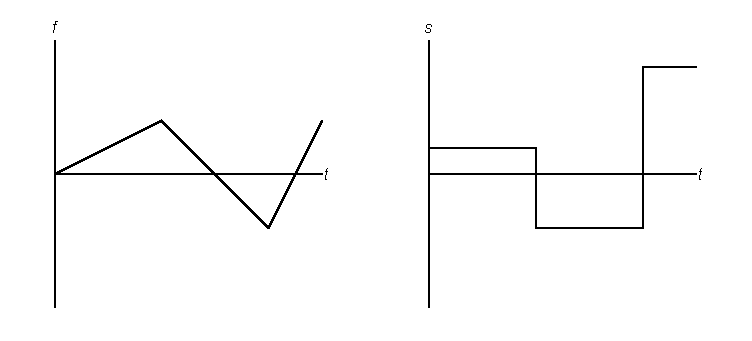
\includegraphics[width=1.0\textwidth]{slopes.pdf}
      \end{figure}
\end{enumerate}
\end{document}